\documentclass[12pt,a4paper]{article}
\usepackage{amsmath,amssymb,mathrsfs,tikz,times,pifont}
\usepackage[T1]{fontenc}
\usepackage{enumitem}
\newcommand\circitem[1]{%
\tikz[baseline=(char.base)]{
\node[circle,draw=gray, fill=red!55,
minimum size=1.2em,inner sep=0] (char) {#1};}}
\newcommand\boxitem[1]{%
\tikz[baseline=(char.base)]{
\node[fill=cyan,
minimum size=1.2em,inner sep=0] (char) {#1};}}
\setlist[enumerate,1]{label=\protect\circitem{\arabic*}}
\setlist[enumerate,2]{label=\protect\boxitem{\alph*}}
%%%::::::by chnini ameur :::::::%%%
\everymath{\displaystyle}
\usepackage[left=1cm,right=1cm,top=1cm,bottom=1.7cm]{geometry}
\usepackage[colorlinks=true, linkcolor=blue, urlcolor=blue, citecolor=blue]{hyperref}
\usepackage{array,multirow}
\usepackage[most]{tcolorbox}
\usepackage{varwidth}
\usepackage{float} %pour utiliser l'option [H] qui force l'image à apparaître exactement à l'endroit où elle est placée dans le code.
\tcbuselibrary{skins,hooks}
\usetikzlibrary{patterns}
%%%::::::by chnini ameur :::::::%%%
\newtcolorbox{exa}[2][]{enhanced,breakable,before skip=2mm,after skip=5mm,
colback=yellow!20!white,colframe=black!20!blue,boxrule=0.5mm,
attach boxed title to top left ={xshift=0.6cm,yshift*=1mm-\tcboxedtitleheight},
fonttitle=\bfseries,
title={#2},#1,
% varwidth boxed title*=-3cm,
boxed title style={frame code={
\path[fill=tcbcolback!30!black]
([yshift=-1mm,xshift=-1mm]frame.north west)
arc[start angle=0,end angle=180,radius=1mm]
([yshift=-1mm,xshift=1mm]frame.north east)
arc[start angle=180,end angle=0,radius=1mm];
\path[left color=tcbcolback!60!black,right color = tcbcolback!60!black,
middle color = tcbcolback!80!black]
([xshift=-2mm]frame.north west) -- ([xshift=2mm]frame.north east)
[rounded corners=1mm]-- ([xshift=1mm,yshift=-1mm]frame.north east)
-- (frame.south east) -- (frame.south west)
-- ([xshift=-1mm,yshift=-1mm]frame.north west)
[sharp corners]-- cycle;
},interior engine=empty,
},interior style={top color=yellow!5}}
%%%%%%%%%%%%%%%%%%%%%%%

\usepackage{fancyhdr}
\usepackage{eso-pic}         % Pour ajouter des éléments en arrière-plan
% Commande pour ajouter du texte en arrière-plan
\usepackage{tkz-tab}
\AddToShipoutPicture{
    \AtTextCenter{%
        \makebox[0pt]{\rotatebox{80}{\textcolor[gray]{0.7}{\fontsize{5cm}{5cm}\selectfont PGB}}}
    }
}
\usepackage{lastpage}
\fancyhf{}
\pagestyle{fancy}
\renewcommand{\footrulewidth}{1pt}
\renewcommand{\headrulewidth}{0pt}
\renewcommand{\footruleskip}{10pt}
\fancyfoot[R]{
\color{blue}\ding{45}\ \textbf{2025}
}
\fancyfoot[L]{
\color{blue}\ding{45}\ \textbf{Prof:M. BA}
}
\cfoot{\bf
\thepage /
\pageref{LastPage}}
\usetikzlibrary{trees} % Bibliothèque pour les arbres
\begin{document}
\renewcommand{\arraystretch}{1.5}
\renewcommand{\arrayrulewidth}{1.2pt}
\begin{tikzpicture}[overlay,remember picture]
\node[draw=blue,line width=1.2pt,fill=purple,text=blue,inner sep=3mm,rounded corners,pattern=dots]at ([yshift=-2.5cm]current page.north) {\begingroup\setlength{\fboxsep}{0pt}\colorbox{white}{\begin{tabular}{|*1{>{\centering \arraybackslash}p{0.28\textwidth}} |*2{>{\centering \arraybackslash}p{0.2\textwidth}|} *1{>{\centering \arraybackslash}p{0.19\textwidth}|} }
\hline
\multicolumn{3}{|c|}{$\diamond$$\diamond$$\diamond$\ \textbf{Lycée de Dindéfélo}\ $\diamond$$\diamond$$\diamond$ }& \textbf{A.S. : 2024/2025} \\ \hline
\textbf{Matière: Mathématiques}& \textbf{Niveau : T}\textbf{S2} &\textbf{Date: 22/05/2025} & \textbf{Durée : 4 heures} \\ \hline
\multicolumn{4}{|c|}{\parbox[c]{10cm}{\begin{center}
\textbf{{\Large\sffamily Correction Composition Du 2$ ^\text{\bf nd} $ Semestre}}
\end{center}}} \\ \hline
\end{tabular}}\endgroup};
\end{tikzpicture}
\vspace{3cm}
\section*{\underline{Exercice 1 :($3$ pts)} Restitution de Connaissances}
\begin{enumerate}
    \item Soit \( \Omega \) l’univers associé à une expérience aléatoire \( E \) et \( p \) une probabilité définie sur \( \Omega \).\\
    Recopie et complète les relations ci-dessous :
    \begin{enumerate}
        \item \( \mathbb{P}(\Omega) = 1 \) \hfill \textbf{(0,25 pt)}
        \item \( \mathbb{P}(\varnothing) = 0 \) \hfill \textbf{(0,25 pt)}
        \item Si \( A \) et \( B \) sont deux événements incompatibles de \( \Omega \), alors \( \mathbb{P}(A \cup B) = \mathbb{P}(A) + \mathbb{P}(B) \) \hfill \textbf{(0,25 pt)}
        \item Soit \( D \) un événement quelconque de \( \Omega \). \( \mathbb{P}(D) = 1{,}5 \) est-il possible ?\\
        \textbf{Non}, car une probabilité est toujours un nombre compris entre 0 et 1. \hfill \textbf{(0,25 pt)}
    \end{enumerate}
    
    \item Soit \( f \) une fonction continue sur un intervalle \( I \) et \( (u_n) \) une suite convergente vers un nombre réel \( L \in I \), définie par \( u_{n+1} = f(u_n) \).\\
    Répondre par vrai ou faux à l’affirmation : \textbf{\( L \) est solution de l’équation \( f(L) = L \)}. \\
    \textbf{Réponse : Vrai} \hfill \textbf{(0,5 pt)}
    
    \item Soit \( (u_n) \) une suite géométrique de raison \( q = \frac{1}{2} \) et de premier terme \( u_2 = -3 \).\\
    Choisir la bonne réponse dans chaque cas : \hfill (\( \textbf{3} \times \textbf{0,25 pt} \))

    \begin{center}
    \renewcommand{\arraystretch}{1.5}
    \begin{tabular}{|>{\centering\arraybackslash}m{5cm}|>{\centering\arraybackslash}m{3cm}|>{\centering\arraybackslash}m{3cm}|>{\centering\arraybackslash}m{3cm}|}
        \hline
        \textbf{Réponses} & \textbf{A} & \textbf{B} & \textbf{C} \\
        \hline
        \( \lim u_n \) est : &  &  & \textbf{X} \\
        \hline
        L’expression de \( u_n \) est : &  &  & \textbf{X} \\
        \hline
        L’expression de \( S_n = u_2 + u_3 + \cdots + u_n \) est : &  & \textbf{X} &  \\
        \hline
    \end{tabular}
    \end{center}

\end{enumerate}

\section*{\underline{Correction de l'Exercice 2 :($3$ pts)}}
Le plan complexe est muni d’un repère orthonormé direct \( (O ; \vec{u}, \vec{v}) \). 

\begin{enumerate}
    \item On considère la transformation \( S \) du plan d’écriture complexe \( z' = (1 - i\sqrt{3})z + 2 \).\\
    On pose \( a = 1 - i\sqrt{3} \) et \( b = 2 \).\\
    Le module de \( a \) est : 
    \[
    |a| = |1 - i\sqrt{3}| = \sqrt{1^2 + (\sqrt{3})^2} = \sqrt{1 + 3} = 2.
    \]
    Donc la transformation est une \textbf{rotation homothétique} (ou similitude directe) de rapport \( 2 \) et d’angle \( \theta \) tel que \( \arg(a) = \arg(1 - i\sqrt{3}) \).\\
    \textbf{Nature de \( S \)} : \boxed{\text{Similitude directe}}. \hfill \textbf{(0,5 pt)}
    
    \item \textbf{Rapport :} \( |a| = 2 \)\\
    \textbf{Argument de \( a \)} :
    \[
    \arg(1 - i\sqrt{3}) = -\arctan\left( \dfrac{\sqrt{3}}{1} \right) = -\dfrac{\pi}{3}.
    \]
    Donc l’angle est \boxed{-\dfrac{\pi}{3}}.\\
    \textbf{Rapport et angle :} \boxed{2 \text{ et } -\dfrac{\pi}{3}}. \hfill \textbf{(0,5 pt)}

    \item Soit \( A \) d’affixe \( z_A = 2 - i\sqrt{3} \). Alors :
    \[
    z'_C = (1 - i\sqrt{3})(2 - i\sqrt{3}) + 2.
    \]
    Développons :
    \[
    z'_C = 2(1) - 2i\sqrt{3} - i\sqrt{3}(1) + (i\sqrt{3})^2 + 2 = 2 - 3i - 3 + 2 = \boxed{-1 - 3i}. \hfill \textbf{(1 pt)}
    \]

    \item \( z_D = -\dfrac{2\sqrt{3}}{3}i \).\\
    On calcule :
    \[
    z'_D = (1 - i\sqrt{3}) \left(-\dfrac{2\sqrt{3}}{3}i \right) + 2.
    \]
    On simplifie :
    \[
    z'_D = -\dfrac{2\sqrt{3}}{3}i + \dfrac{2\cdot 3}{3} = -\dfrac{2\sqrt{3}}{3}i + 2.
    \]
    Donc \boxed{z'_D = 2 - \dfrac{2\sqrt{3}}{3}i}. \hfill \textbf{(0,75 pt)}\\
    Interprétation : \( D \) est un point situé sur le \textbf{cercle de centre} le centre de la similitude et de rayon proportionnel à son image. Ce n’est ni un point fixe ni un invariant remarquable ici.\\
    Autre interprétation : comme l’image n’est pas identique à \( D \), \boxed{D \text{ n’est pas un point invariant de } S}. \hfill \textbf{(0,25 pt)}
\end{enumerate}

\section*{\underline{Exercice 3 :($4$ pts)} }
\begin{enumerate}
    \item Construisons un arbre pondère correspondant à cette épreuve.
% Styles pour les différents niveaux de l'arbre
\tikzstyle{level 1}=[level distance=2.9cm, sibling distance=7cm] % Niveau 1 : distance verticale et entre branches
\tikzstyle{level 2}=[level distance=3.5cm, sibling distance=3cm] % Niveau 2 : plus resserré
\tikzstyle{bag} = [text centered] % Style pour les nœuds intermédiaires
\tikzstyle{end} = [text centered] % Style pour les feuilles
\definecolor{darkgreen}{RGB}{0,100,0} % Couleur vert foncé (non utilisée ici)
\definecolor{darkred}{RGB}{139,0,0} % Couleur rouge foncé

\begin{tikzpicture}[grow=right, sloped] % Arbre qui se développe vers la droite, étiquettes inclinées

% Nœud racine (départ de l'univers)
\node[bag] {\textcolor{darkred}{}} 
    child {
        % Première branche : événement B
        node[bag] {\textcolor{darkred}{$N_1$}} 
            child {
                % Sous-branche de B : issue V
                node[end] {\textcolor{darkred}{$R_2$}} 
                edge from parent
                node[above] {\textcolor{black}{$\frac{1}{5}$}} % Probabilité conditionnelle : P(V|B)
            }
            child {
                % Sous-branche de B : issue M
                node[end] {\textcolor{darkred}{$N_2$}} 
                edge from parent
                node[above] {\textcolor{black}{$\frac{3}{5}$}} % Probabilité à compléter
            }
            child {
                % Sous-branche de B : issue R
                node[end] {\textcolor{darkred}{$B_2$}} 
                edge from parent
                node[above] {\textcolor{black}{$\frac{1}{5}$}} % Probabilité à compléter
            }
        edge from parent
        node[above] {\textcolor{black}{$\frac{6}{9}$}} % Probabilité de B : P(B)
    }
    child {
        % Deuxième branche : événement A
        node[bag] {\textcolor{darkred}{$B_1$}} 
            child {
                % Sous-branche de A : issue V
                node[end] {\textcolor{darkred}{$R_2$}} 
                edge from parent
                node[above] {\textcolor{black}{$\frac{1   }{5}$}} % Probabilité à compléter
            }
            child {
                % Sous-branche de A : issue M
                node[end] {\textcolor{darkred}{$N_2$}} 
                edge from parent
                node[above] {\textcolor{black}{$\frac{2   }{5}$}} % Probabilité à compléter
            }
            child {
                % Sous-branche de A : issue R
                node[end] {\textcolor{darkred}{$B2$}} 
                edge from parent
                node[above] {\textcolor{black}{$\frac{2}{5}$}} % Probabilité conditionnelle : P(R|A)
            }
        edge from parent
        node[above] {\textcolor{black}{$\frac{3}{9}$}} % Probabilité de A : P(A), à compléter
    };
\end{tikzpicture}
\item Montrons que $P(N_{2}) = \frac{8}{15}$
\begin{enumerate}
    \item $P(N_{2})$ peut être calculé par la loi des totalisations :

    \(
    \begin{aligned}
        P(N_2) &= P(N_2 | B_1) \cdot P(B_1) + P(N_2 | N_1) \cdot P(N_1)\\
               &= \left( \frac{2}{5} \cdot \frac{1}{3} \right) + \left( \frac{3}{5} \cdot \frac{2}{3} \right)\\
               &= \frac{2}{15} + \frac{6}{15}\\
               &= \frac{8}{15}
    \end{aligned}
    \)
    \item Déterminons la probabilité de l'événement $B_{2}$

    \(
    \begin{aligned}
        P(B_2) &= P(B_2 | B_1) \cdot P(B_1) + P(B_2 | N_1) \cdot P(N_1)\\
               &= \left( \frac{1}{5} \cdot \frac{1}{3} \right) + \left( \frac{1}{5} \cdot \frac{2}{3} \right)\\
               &= \frac{1}{15} + \frac{2}{15}  \\
               &= \frac{3}{15}\\
               &= \frac{1}{5}
    \end{aligned}
    \)
    \item Déterminons la probabilité de tirer une boule blanche de $u_{1}$, sachant que la boule tirée dans $u_{2}$ est noire
On utilise le théorème de Bayes :\\
 \(
    \begin{aligned}
        P(B_1 | N_2) &= \frac{P(N_2 | B_1) \cdot P(B_1)}{P(N_2)}\\
                    &=  \frac{\left( \frac{2}{5} \right) \cdot \left( \frac{1}{3} \right)}{\frac{8}{15}}\\
                    &= \frac{\frac{2}{15}}{\frac{8}{15}}  \\
                    &= \frac{2}{8}\\
                    &= \frac{1}{4}
    \end{aligned}
    \)
\end{enumerate}
\item 
\begin{enumerate}
    \item Loi de probabilité de $X$ Nous avons les différents gains :
\begin{itemize}
    \item Boule blanche dans $u_{2}$ : $3000F - 500F = 2500F$
    \item Boule noire dans $u_{2}$ : $0F - 500F = -500F$
    \item Boule rouge dans $u_{2}$ : $500F - 500F = 0F$
\end{itemize}

Calcul des probabilités de $X$ :
\begin{itemize}
    \item $P(X = 2500) = P(B_{2}) = \frac{1}{5}$
    \item $P(X = -500) = P(N_{2}) = \frac{8}{15}$
    \item $P(X = 0) = P(R) = \left( \frac{2}{5} \cdot \frac{1}{3} \right) + \left( \frac{1}{5} \cdot \frac{2}{3} \right) = \frac{4}{15}$
\end{itemize}    

    \item Calculons de l'espérance mathématique, Variance et écart-type de $X$ et écart-type de $X$
    \begin{itemize}
        \item \textbf{Espérance mathématique}
    
    \(
    \begin{aligned}
        E(X) &= 2500 \cdot P(X = 2500) + (-500) \cdot P(X = -500) + 0 \cdot P(X = 0)\\
             &= 2500 \cdot \frac{1}{5} + (-500) \cdot \frac{8}{15} + 0 \cdot \frac{4}{15}\\
             &= 500 - \frac{4000}{15}\\
             &= \frac{7500 - 4000}{15}\\
             &=\frac{3500}{15} \\
             &\approx 233.33
    \end{aligned}
    \)
    
        \item \textbf{Variance de $X$}

    \(
    \begin{aligned}
        Var(X) &= E(X^2) - (E(X))^2\\
    \end{aligned}
    \)

    \(
    \begin{aligned}
        E(X^2) &= (2500^2) \cdot P(X = 2500) + (-500)^2 \cdot P(X = -500) + 0^2 \cdot P(X = 0)\\
               &= 6250000 \cdot \frac{1}{5} + 250000 \cdot \frac{8}{15}\\
               &= 1250000 + \frac{2000000}{15}\\
               &= 1250000 + \frac{133333.33}{1}\\ 
               &\approx 1383333.33
    \end{aligned}
    \)
    
Donc, 

\(
    \begin{aligned}
        Var(X) &= E(X^2) - (E(X))^2\\
               &= 1383333.33 - (233.33)^2\\
               &\approx 1383333.33 - 54444.44\\
               &\approx 1338898.89\\ 
    \end{aligned}
\)

        \item  \textbf{Ecart-type $X$}

$\sigma(X)$ est $\sigma(X) = \sqrt{Var(X)}$
    \end{itemize}
    \item Déterminons la fonction de répartition de X et représentons la.

\[
F(x) = \mathbb{P}(X \leq x)
\]

\[
F(x) =
\begin{cases}
0 & \text{si } x \in ]{-\infty}, -500[ \\
\dfrac{8}{15} & \text{si } x \in [-500,\; 0[ \\
\dfrac{11}{15} & \text{si } x \in [0,\; 2500[ \\
1 & \text{si } x \in [2500,\; +\infty[
\end{cases}
\]


\end{enumerate}
\item Calculons cela pour trouver le nombre minimal de parties.
Soit \( p = P(N_2) = \dfrac{8}{15} \). On veut trouver le plus petit entier \( n \) tel que :
\[
1 - (1 - p)^n > 0{,}97
\]
\[
(1 - \dfrac{8}{15})^n < 0{,}03 \quad \text{soit} \quad \left( \dfrac{7}{15} \right)^n < 0{,}03
\]
\[
n \log\left( \dfrac{7}{15} \right) < \log(0{,}03)
\]
\[
n > \dfrac{\log(0{,}03)}{\log\left( \dfrac{7}{15} \right)} \approx 6{,}6
\]

\textbf{Donc } \( n = 7 \)

\end{enumerate}
\section*{\underline{Problème :}\quad\textbf{10 pts}}
\section*{Partie A}

On considère la fonction \( g \) définie sur \( ]0; +\infty[ \) par
\[
g(x) = \ln\left( \frac{x+1}{x} \right) - \frac{1}{x+1}.
\]

\bigskip

\textbf{1. Calcul des limites}

\(
\begin{aligned}
\lim_{x \to 0^{+}} g(x) 
&= \lim_{x \to 0^{+}} \ln\left( \frac{x+1}{x} \right) - \lim_{x \to 0^{+}} \frac{1}{x+1} \\
&= +\infty - 1 \\
&= +\infty,\text{ puisque }  \frac{x+1}{x} \to +\infty  \text{ quand } x \to 0^{+}
\end{aligned}
\)

\(
\begin{aligned}
\lim_{x \to +\infty} g(x) 
&= \lim_{x \to +\infty} \ln\left( 1 + \frac{1}{x} \right) - \lim_{x \to +\infty} \frac{1}{x+1} \\
&= 0 - 0 \\
&= 0.
\end{aligned}
\)

\bigskip

\textbf{2. Étude des variations et tableau}

\(
\begin{aligned}
    g'(x) &= \ln\left( \frac{x+1}{x} \right)' - \left(\frac{1}{x+1}\right)'\\
          &= \frac{(x+1)'}{x+1} - \frac{x'}{x} + \frac{(x+1)'}{(x+1)^2}\\
          &= \frac{1}{x+1} - \frac{1}{x} + \frac{1}{(x+1)^2}\\
          &= \frac{x(x+1) - (x+1)^2 + x}{x(x+1)^2}\\
          &= \frac{x(x+1) - (x+1)^2 + x}{x(x+1)^2}\\
          &= \frac{x^2 + x - (x^2 + 2x + 1) + x}{x(x+1)^2}\\
          &= \frac{-1}{x(x+1)^2}
\end{aligned}
\)

Ainsi,
\[
g'(x) = \frac{-1}{x(x+1)^2} < 0 \quad \text{pour tout } x > 0.
\]

\bigskip

\textbf{Tableau de variations de \( g \) sur \( ]0; +\infty[ \)}

    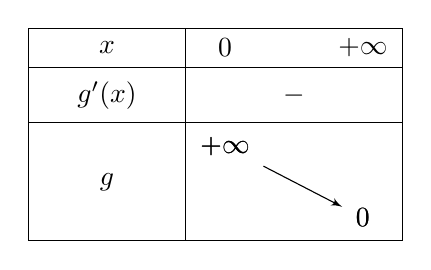
\begin{tikzpicture}[node style/.style={fill opacity=0,text opacity=1}]
        \tkzTabInit[espcl=1.75]{$x$/.5,$g'(x)$/.7,$g$/1.5}{$0$,$+\infty$}
        \tkzTabLine{,-,}
        \tkzTabVar{+/$+\infty$,-/$0$/}
    \end{tikzpicture}

\bigskip

\textbf{3. Signe de \( g(x) \) sur \( ]0; +\infty[ \)}

Comme \( g \) est strictement décroissante et tend vers 0 par la droite quand \( x \to +\infty \), et part de \( +\infty \) à 0, on en déduit que
\[
g(x) > 0 \quad \text{pour tout } x > 0.
\]

\section*{Partie B}

Soit la fonction \( f \) définie par :
\[
f(x) = 
\begin{cases}
x \ln\left( \dfrac{x+1}{x} \right) + 1 & \text{si } x > 0, \\[6pt]
(x^2 - 3x + 1)\, e^x & \text{si } x \leq 0.
\end{cases}
\]

\begin{enumerate}
\item 
    \begin{enumerate}
        \item Domaine de définition de \( f \)
        Pour \( x > 0 \), \( \dfrac{x+1}{x} = 1 + \dfrac{1}{x} > 1 \), donc le logarithme est défini. La fonction est donc définie sur cet intervalle.
     
        Pour \( x \leq 0 \), l'expression est polynomiale multipliée par une exponentielle : bien définie sur tout \( \mathbb{R} \).
     
        Par conséquent, la fonction \( f \) est définie sur \( \mathbb{R} \).

        \item Limites aux bornes du domaine
        
        \textbf{Limite en \( -\infty \)} :

        \( \lim\limits_{x \to -\infty} (x^2 - 3x + 1)\, e^x = 0, \)
         car \( e^x \to 0 \) plus vite que toute puissance.

         \textbf{Limite en \( +\infty \)} :

         \(\text{ Posons } X=\dfrac{x+1}{x} \text{ donc } x=\dfrac{1}{X-1} \text{ Si } x\to +\infty \text{ alors } X \to 0\)

         \(
            \begin{aligned}
                \lim\limits_{x \to +\infty}f(x)&=\lim\limits_{x \to +\infty}x \ln\left( \dfrac{x+1}{x} \right) + 1\\
                &=\lim\limits_{X \to 0}\dfrac{1}{X-1} \ln\left( X \right) + 1\\
                &=\lim\limits_{X \to 0}\dfrac{\ln\left( X \right)}{X-1}  + 1\\
                &=1  + 1\\
            \end{aligned}
        \)
        
         Ainsi : \(\lim\limits_{x \to +\infty} f(x) = 2.\)
        \item Asymptotes
        \begin{itemize}
            \item En \( -\infty \), la limite est 0, donc asymptote horizontale : \( y = 0 \).
            \item En \( +\infty \), la limite est 2, donc asymptote horizontale : \( y = 2 \).
\end{itemize}
    \end{enumerate} 
    \textbf{Conclusion :} La fonction admet deux asymptotes horizontales : \( y = 0 \) en \( -\infty \), et \( y = 2 \) en \( +\infty \).
    \item 
    \begin{enumerate}
        \item \textbf{Continuité de \( f \) en 0.} \hfill \textbf{(0,75 pt)}
        
        \textbf{\underline{En $0^-$}:}
        
        \(
        \begin{aligned}
            \lim\limits_{x \to 0^-} f(x) &= \lim\limits_{x \to 0^-} (x^2 - 3x + 1)\, e^x\\
            &= 1
        \end{aligned}
        \)

        \textbf{\underline{En $0^+$}:}
        
        \(
            \begin{aligned}
                \lim\limits_{x \to 0^+} f(x) &= \lim\limits_{x \to 0^+} \left( x \ln\left( \frac{x+1}{x} \right) + 1 \right)\\
                &= 1
            \end{aligned}
        \)
        
        De plus, \(f(0) = (0^2 - 3 \cdot 0 + 1)\, e^0 = 1.\)
        
        Donc \( \lim\limits_{x \to 0^-} f(x) = \lim\limits_{x \to 0^+} f(x) = f(0) = 1\)
        
        ce qui prouve que \( f \) est \textbf{continue en 0}.

        \item \textbf{Dérivabilité de \( f \) en 0 et interprétation des résultats.} \hfill \textbf{(0,75 + 0,25 pt)}

        Pour \( x \leq 0 \), on a : \( f(x) = (x^2 - 3x + 1) e^x. \)
        
        \( 
        \begin{aligned}
            \lim\limits_{x \to 0^-}\frac{f(x)-f(0)}{x-0} &= \lim\limits_{x \to 0^-}\frac{(x^2 - 3x + 1) e^x-1}{x}\\
            &= \lim\limits_{x \to 0^-}\frac{(x^2 - 3x + 1) e^x-1}{x}\\
            &= \lim\limits_{x \to 0^-} \frac{(x^2 - 3x)\, e^x + (e^x - 1)}{x} \\
            &= \lim\limits_{x \to 0^-} (x - 3)\, e^x + \lim\limits_{x \to 0^-} \frac{e^x - 1}{x} \\
            &= -3 + 1 \\
            &= -2.
        \end{aligned}
        \)

    \(\lim\limits_{x \to 0^-}\frac{f(x)-f(0)}{x-0}=-2\)

        Pour \( x > 0 \), on a : \(f(x) = x \ln\left( \dfrac{x+1}{x} \right) + 1.\)

        \( 
        \begin{aligned}
            \lim\limits_{x \to 0^+} \frac{f(x) - f(0)}{x}&= \lim\limits_{x \to 0^+} \frac{x \ln\left( \dfrac{x+1}{x} \right)+1-1}{x} \\
            \lim\limits_{x \to 0^+} \frac{f(x) - f(0)}{x}&= \lim\limits_{x \to 0^+} \frac{x \ln\left( \dfrac{x+1}{x} \right)}{x} \\
            &= \lim\limits_{x \to 0^+} \ln\left( \dfrac{x+1}{x} \right) \\
            &= \lim\limits_{x \to 0^+} \ln\left( 1 + \dfrac{1}{x} \right)\\
            &= +\infty
        \end{aligned}
        \)

\(  \lim\limits_{x \to 0^-} \frac{f(x) - f(0)}{x} \neq \lim\limits_{x \to 0^+} \frac{f(x) - f(0)}{x}\) donc \( f \) n’est \textbf{pas dérivable en 0}.

        \textbf{Interprétation :}

\begin{itemize}
    \item En \( 0^- \) : \( \displaystyle \lim\limits_{x \to 0^-} \frac{f(x) - f(0)}{x} = -2 \)  
    donc la courbe \( \mathcal{C}_f \) admet une \textbf{demi-tangente} à gauche d'équation : \( y = -2x + 1 \)

    \item En \( 0^+ \) : \( \displaystyle \lim\limits_{x \to 0^+} \frac{f(x) - f(0)}{x} = +\infty \)  
    donc la courbe \( \mathcal{C}_f \) admet une \textbf{demi-tangente verticale orientée vers le haut} à droite.
\end{itemize}
    \end{enumerate}
\item \textbf{Montrons que } 
\(
f'(x) = 
\begin{cases}
g(x) & \text{si } x > 0 \\
(x^2 - x - 2)\, e^x & \text{si } x < 0
\end{cases}
\) \hfill \textbf{(1 pt)}

\(
    f(x) = 
\begin{cases}
x \ln\left( \dfrac{x+1}{x} \right) + 1 & \text{si } x > 0, \\
(x^2 - 3x + 1)\, e^x & \text{si } x \leq 0.
\end{cases}
\)

\(
\begin{aligned}
    f'(x) = 
\begin{cases}
 \left[x\ln\left( \dfrac{x+1}{x} \right) + 1\right]' \\
\left[(x^2 - 3x + 1)\, e^x\right]' 
\end{cases}
&\implies
\begin{cases}
 \ln\left( \dfrac{x+1}{x} \right)+x\left[\frac{1}{x+1}-\frac{1}{x}\right] \\
\left( x^2 - 3x + 1 \right)' e^x + \left( x^2 - 3x + 1 \right) (e^x)'
\end{cases}\\
&\implies
\begin{cases}
 \ln\left( \dfrac{x+1}{x} \right)+\frac{x}{x+1}-1\\
\left( 2x - 3 + x^2 - 3x + 1 \right) e^x
\end{cases}\\
&\implies
\begin{cases}
 \ln\left( \dfrac{x+1}{x} \right)-\frac{1}{x+1}\\
 (x^2 - x - 2)\, e^x 
\end{cases}
\end{aligned}
\)

\textbf{Conclusion :} On a bien :
\[
f'(x) = 
\begin{cases}
g(x) & \text{si } x > 0 \\
(x^2 - x - 2)\, e^x & \text{si } x < 0
\end{cases}
\]
\item Tableau de variation

\(f'(x) = (x^2 - x - 2)\, e^x\)

Comme \( e^x > 0 \) pour tout réel, le signe de \( f'(x) \) est celui du polynôme :\(P(x) = x^2 - x - 2\)

On résout \( P(x) = 0 \) :
\[
x^2 - x - 2 = 0 \quad \Longleftrightarrow \quad x = -1 \quad \text{ou} \quad x = 2
\]

On dresse le tableau de signes de \( P(x) \), mais en restreignant à \( x < 0 \) :

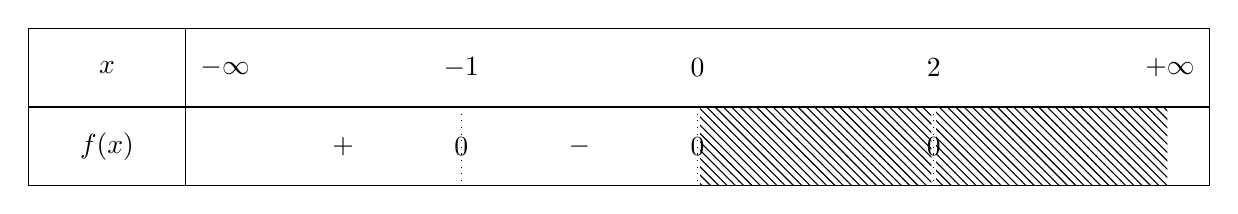
\begin{tikzpicture}
   \tkzTabInit{$x$ / 1 , $f(x)$ / 1}{$-\infty$, $-1$,$0$, $2$, $+\infty$}
   \tkzTabLine{, +, z,-, z, h, z,h }
\end{tikzpicture}

\begin{itemize}
    \item Pour \( x < -1 \), \( f'(x) > 0 \), donc \( f \) est \textbf{croissante}.
    \item Pour \( -1 < x < 0 \), \( f'(x) < 0 \), donc \( f \) est \textbf{décroissante}.
    \item Pour \( x > 0 \), on a montré que \( f'(x) = g(x) > 0 \), donc \( f \) est \textbf{croissante}.
\end{itemize}

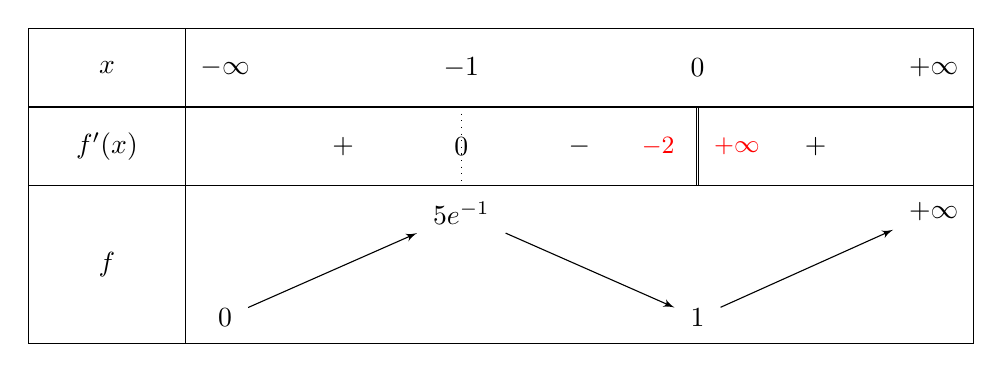
\begin{tikzpicture}
   \tkzTabInit{$x$ / 1 ,  $f'(x)$ / 1 ,  $f$ / 2}{$-\infty$, $-1$, $0$, $+\infty$}
   \tkzTabLine{,+, z, -, d, +}
   \tkzTabVar{-/$0$, +/$5e^{-1}$, -/$1$, +/$+\infty$}

   % Ajout des pentes avec des nodes au-dessus de la ligne des variations
   \node[text=red] at (8, -1.5) {\small\(-2\)};
   \node[text=red] at (9, -1.5) {\small\(+\infty\)};
\end{tikzpicture}
\section*{Partie C : \textbf{2,5 pts}}

Soit \( h \) la restriction de \( f \) à l’intervalle \( ]0 ; +\infty[ \) :
\[
h(x) = x \ln\left( \dfrac{x+1}{x} \right) + 1
\]

    \item Montrons que \( h \) est bijective de \( ]0 ; +\infty[ \) vers un intervalle \( J \). \hfill \textbf{(0,5 pt)}

    On a déjà montré que \( f \) est strictement croissante sur \( ]0 ; +\infty[ \) car \( f'(x) = g(x) > 0 \).\\
    Ainsi, \( h \) est continue et strictement croissante sur \( ]0 ; +\infty[ \), donc \textbf{bijective}.\\

    D'autre part :
    \[
    \lim_{x \to 0^+} h(x) = 1 \quad \text{et} \quad \lim_{x \to +\infty} h(x) = 2
    \]

    Donc :
    \[
    \boxed{h : \, ]0 ; +\infty[ \to ]1 ; 2[, \text{ bijection}}
    \]

    \item Étudier la dérivabilité de \( h^{-1} \) sur \( J \). \hfill \textbf{(0,5 pt)}

    \( h'(x) = g(x) > 0 \) sur \(]0 ; +\infty[\).\\
    Donc \( h \) est dérivable, strictement croissante, et \( \forall x \in ]0 ; +\infty[\) \( h'(x) \ne 0 \), donc sa réciproque est dérivable sur \( J = ]1 ; 2[ \).\\

    \boxed{h^{-1} \text{ est dérivable sur } J, \text{ avec } (h^{-1})'(y) = \dfrac{1}{g(h^{-1}(y))}}

    \item Tracer sur le même graphe les asymptotes, \( \mathcal{C}_f \) et \( \mathcal{C}_{h^{-1}} \). \hfill \textbf{(1,5 pt)}

	    \begin{center}
        \begin{figure}[H]% Forcer l'image à cet endroit
         \centering
         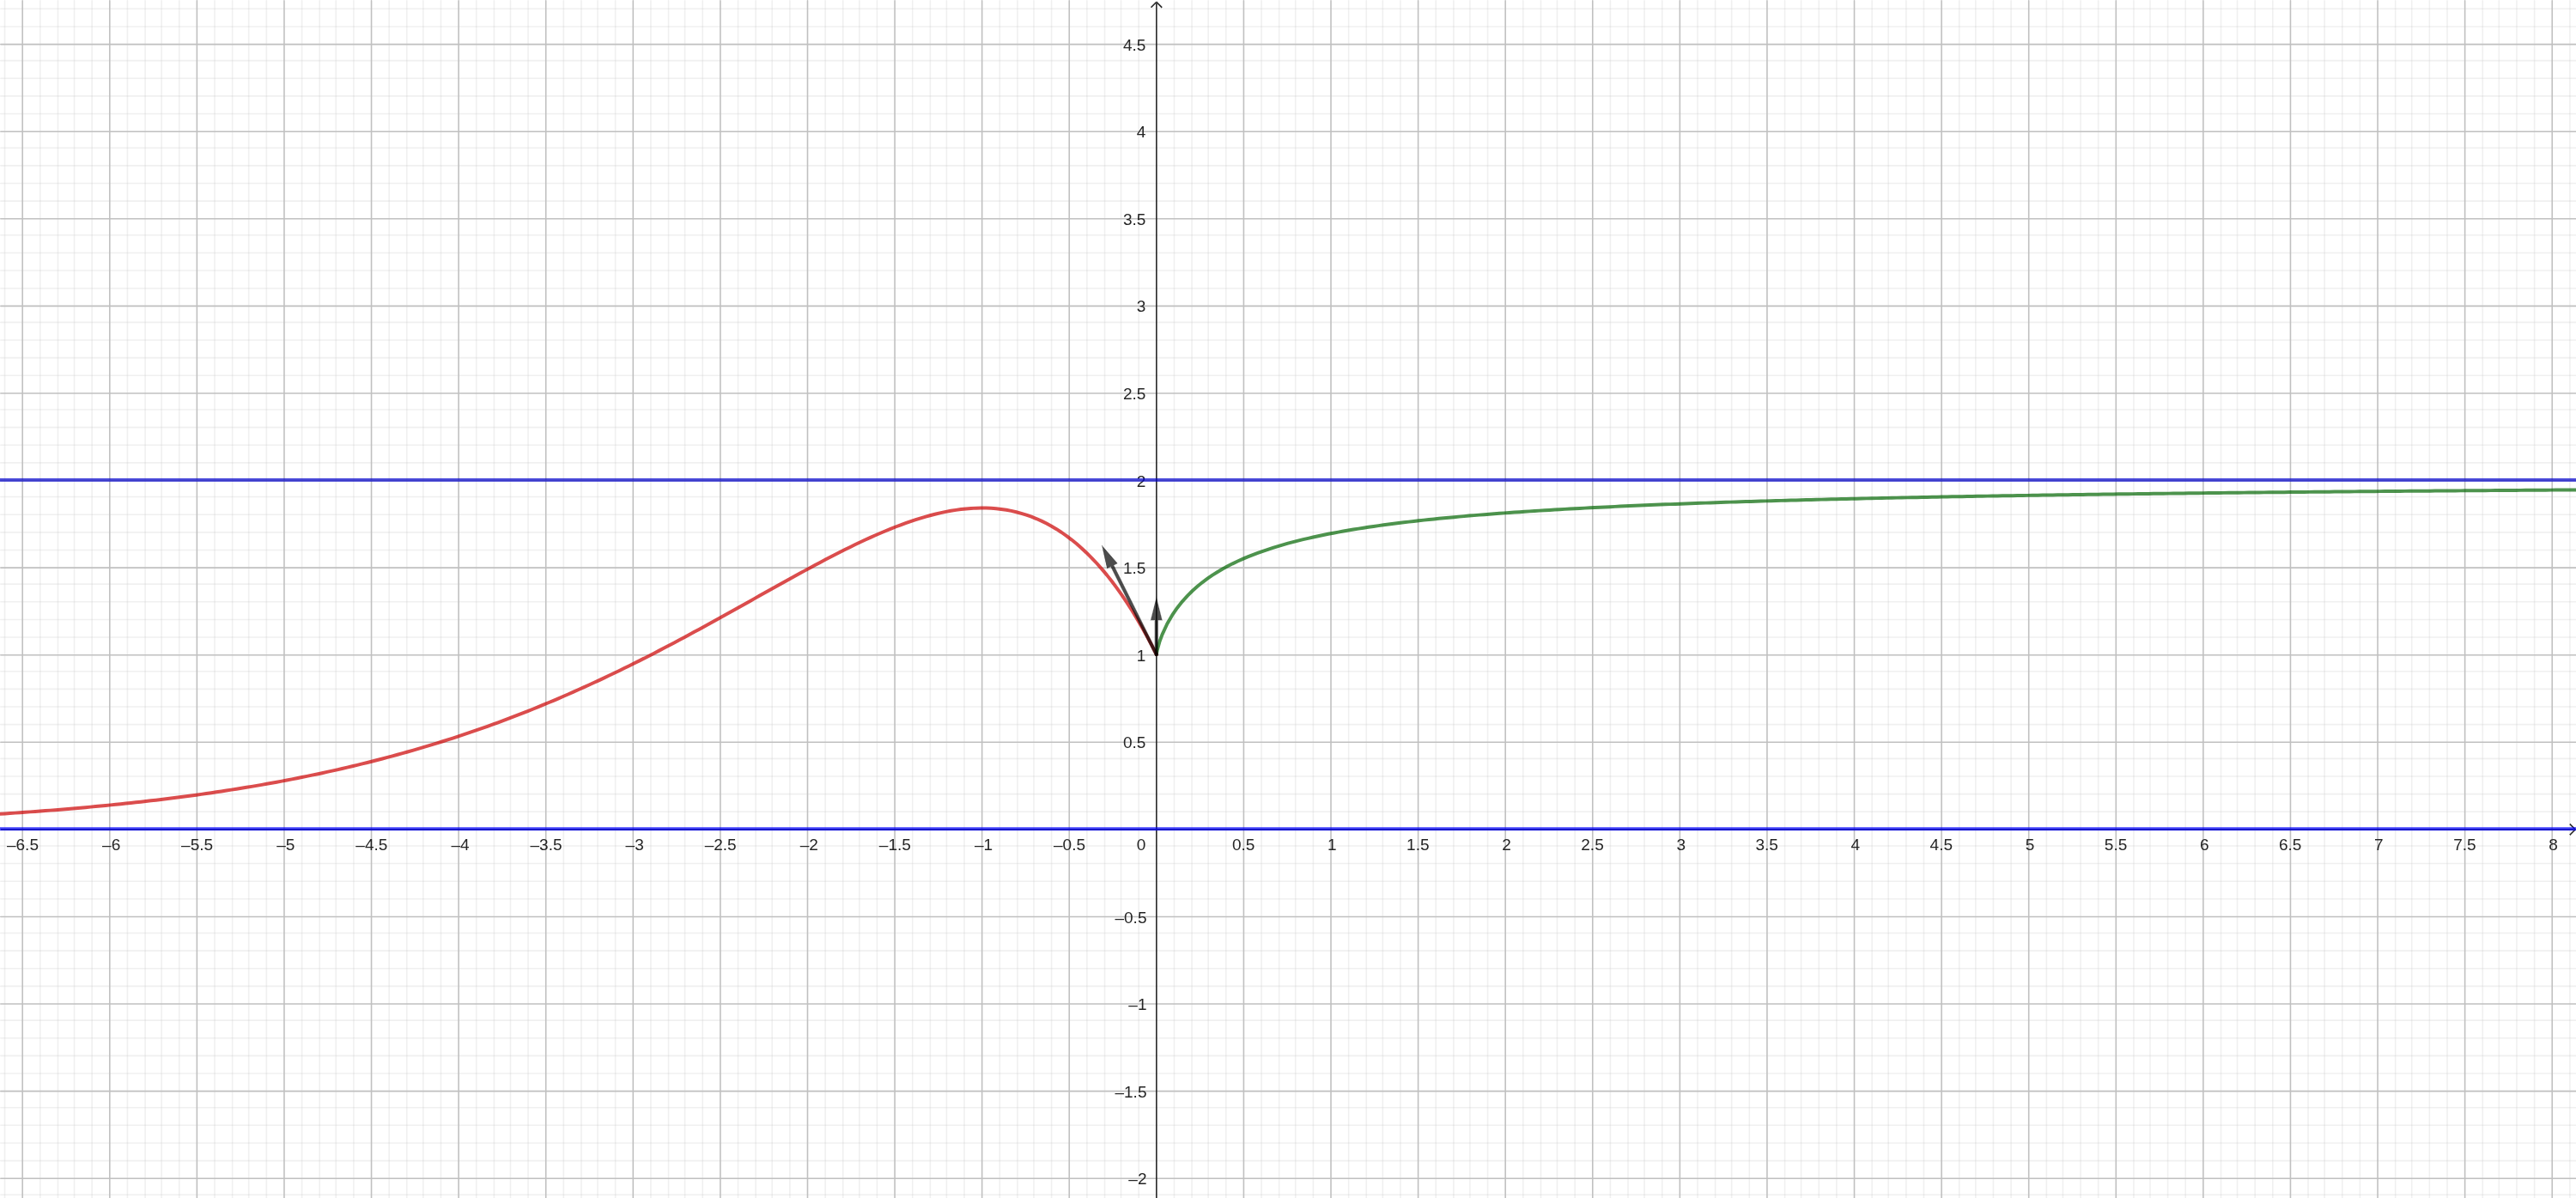
\includegraphics[width=0.8\textwidth]{Compo2.png}
        \end{figure}
    \end{center}
        \href{https://www.geogebra.org/classic/kgbuagda}{Clique ici pour voir la figure sur géogébra}
\end{enumerate}
    
\end{document}
